%!TEX root = ../dissertation.tex
\begin{savequote}[75mm]
This is some random quote to start off the chapter.
\qauthor{Firstname lastname}
\end{savequote}

\chapter{Continuous adaption for communication}
\graphicspath{{./figures/modeling/}}

\section{A hierarchical Bayesian perspective on communication (from CADA)}

Hierarchical Bayesian models have been key to quantitatively explaining how the human mind solves difficult inductive problems in domains like causal learning and concept learning where idiosyncratic particulars of instances must be jointly inferred with knowledge that is shared across instances \shortcite{tenenbaum_how_2011}.
For instance, the concept of a ``dog'' abstracts away from our experiences with different instances of dogs across a lifetime, and provides stable expectations about the properties of a new instance -- four legs, wagging tail, barking noises.

%More than the relatively fixed, biological concept of a dog, though, language can be seen as a moving target. The only data we use to ground our learning is produced by other agents who are in the same position as we are, and our only goal is to coordinate on the same meanings in context. This is the sense in which the meanings we learn are conventional. 
However, extensive experience with a particular dog \emph{Fido} reveals idiosyncratic properties, like the pattern of spots on his coat.
This example from concept learning can be adapted as a novel perspective on how conventions work: accumulated knowledge about linguistic conventions in one's community provides stable communicative ``priors'' that guide how we approach new partners, but the language we use to talk with a family member or close collaborator may deviate considerably from the usage predicted by population-level conventions.

Hierarchical Bayesian models thus provide a formal method for both smoothly integrating population-level expectations with partner-specific ones, and also appropriately \emph{updating} population-level knowledge through additional partner-specific observations. 

We begin by proposing a hierarchical Bayesian model of convention formation \cite{GelmanEtAl14_BDA,TenenbaumKempGriffithsGoodman11_Grow_a_Mind_Science} that provides a useful mathematical and conceptual framework for addressing these challenges. Hierarchical models have been key to explaining how the human mind solves difficult inductive problems in domain like causal learning \cite{KempGoodmanTenenbaum10_LearningToLearn,GoodmanUllmanTenenbaum11_TheoryOfCausality} and concept learning \cite{KempPerforsTenenbaum07_HBM} where abstract, shared properties must be jointly inferred with idiosyncratic particulars of instances. More than the relatively fixed, biological concept of a dog, though, language is a moving target. The only data we use to ground our learning is produced by other agents who are in the same position as we are, and our only goal is to coordinate on the same meanings in context \cite{HassonGhazanfar___Keysers12BrainToBrain}. This is the sense in which the meanings we learn are conventional. This \emph{social grounding} is precisely what gives rise to the fascinating idiosyncracies of local convention formation.

We begin by defining a lexicon as a function $$\mathcal{L}_i: (w, o) \rightarrow [0,1]$$ assigning any word-object pair a real-valued meaning in the unit interval \cite{GrafEtAl16_BasicLevel}\footnote{
We mostly have nouns (\emph{poodle, animal, John}) and property adjectives (\emph{blue, squiggly, delicious}) in mind here, which can be assigned direct semantic meanings. How tricker cases like relational modifiers (\emph{some, barely, former}) are represented in the mental lexicon and how to build a fully compositional semantics from them is a topic of ongoing work in formal semantics, though see \citeA{Yildirim16_TalkerSpecificityQuantifiers} for a study exploring how these too can adapt in partner-specific ways over repeated interaction.
}. There are \emph{many} potential ways this function could be represented in the mind at the algorithmic level. It could be derived from a store of exemplars, a set of independent prototypes for each word, a neural network embedding words and objects in a vector space, and so on \cite<see>[for a recent review of candidates]{JonesEtAl15_SemanticMemory}.

Just as our concept of a dog, built up over many individual experiences across a lifetime, provides stable expectations about the properties of a new instance -- four legs, wagging tail, barking noises -- our accumulated lexical knowledge provides stable communicative expectations. 
This knowledge is represented by a `overhypothesis' or shared lexical representation $\Theta_0$, which parameterizes the prior expectations about any individual partner's lexicon: $P(\mathcal{L}_i | \Theta_0)$. 

For the conceptual purposes of this paper, it is not important exactly what form this distribution takes, or what initial prior over the overhypothesis $P(\Theta_0)$ could in principle guide early language learning
\footnote{
For simplicity, we could assume $\Theta_0$ is an $\mathcal{W} \times \mathcal{O} \times 2$ tensor containing values $(\alpha_{(w,o)}, \beta_{(w,o)})$ for every entry $(w,o)$ in the lexicon $\mathcal{L}_i$. This would factor the lexical prior $P(\mathcal{L}_i | \Theta_0)$ into independent Beta distributions over intervals $[0,1]$. It would then be straightforward to place an uninformative prior $P(\Theta_0)$ over that tensor which does not overwhelm the likelihood \cite<see>[p. 110, for some reasonable choices]{GelmanEtAl14_BDA}. More generally, we could allow for arbitrarily complex dependencies between entries of the lexicon by using a Bayesian neural network with weight tensor $\Theta_0$.% that takes word-object pairs $(w,o)$ as input. 
}. It only matters that this knowledge is hierarchical: we expect all members of our language community to share some commonality in what they mean by things. 

Now that we have defined a hierarchical likelihood on lexical beliefs, we must say how we \emph{learn} partner-specific models. Just as years of living with your beloved Fido reveals properties which deviate from your general dog concept -- patches of hair missing from his legs, an odd squeaking noise he makes when excited -- the language we use to talk with a family member or close collaborator may deviate considerably from the usage predicted by global conventions. In other words, our beliefs about a particular partner's lexicon $\mathcal{L}_i$ are formed by integrating our abstract lexical knowledge $\Theta_0$ with particular  observations $D_i$ of that particular individual:
$$%\begin{array}{rcl}
P(\mathcal{L}_i | D_i)  \propto \int_{\Theta_0}P(\mathcal{L}_i | D_i,  \Theta_0) P(\Theta_0 | D_i) 
%                     & = & \mathbb{E}_{\Theta_0}[P(\mathcal{L}_i | \Theta_0, D_i)] 
%\end{array}
$$
where the posteriors in the integral can be computed using Bayes rule:
$$
P(\mathcal{L}_i | D_i, \Theta_0) \propto P(D_i | \mathcal{L}_i, \Theta_0) P(\mathcal{L}_i | \Theta_0)
$$
While this holds when we only have observations from a single speaker, note that our posterior beliefs about $\Theta_0$ are in fact informed by observations from \emph{all} speakers: $D = \bigcup_{i=1}^k D_i$. For  adult language users who have observed innumerable uses of language over their lifetimes, the contribution of a new data point to the overhypothesis $P(\Theta_0 | D)$ should be negligible; the contribution to a partner-specific model, however, can be quite strong. 

Finally, to fully specify our model and compute our partner-specific lexical posterior $P(\mathcal{L}_i, D_i, \Theta_0)$, we must link our beliefs about a partner's lexica to their actual behavior with a likelihood function $P(D_i | \mathcal{L}_i, \Theta_0)$. This is naturally supplied by the Rational Speech Act framework \cite{FrankGoodman12_PragmaticReasoningLanguageGames,GoodmanFrank16_RSATiCS,BergenLevyGoodman16_LexicalUncertainty,SmithGoodmanFrank13_RecursivePragmaticReasoningNIPS}: we assume speakers produce utterances that are parsimonious yet informative in context with respect to their lexicon, and listeners interpret utterances by inverting a speaker model. Because we expect our partner to use language rationally given some lexicon, the utterance they choose to refer to some object will be probable under some lexica and highly improbable under others. In this way, a particular agent's language use is a cue to their particular lexicon. We omit mathematical details here due to the conceptual nature of the article, but a full account of the non-hierarchical version of this model can be found in \citeA{HawkinsFrankGoodman17_ConventionFormation}.

In summary, our hierarchical model formalizes the intuition that global conventions are learned and generalized over many extended interactions with many different people across a lifetime, and that this shared semantic prototype is the backbone supporting rapid learning for new partners and situations. 


\subsection{From grant (maybe cleaner than above?)}
This model will extend the non-hierarchical Bayesian model of \emph{partner-specific} adaptation I developed in my dissertation work \shortcite{hawkins_convention-formation_2017, hawkins_emerging_abstractions_2018} to multiple partners, thus providing the first opportunity to test how collective patterns emerge from rich, repeated interactions with known partners in a community. 
Here I sketch the ``ideal'' mathematical form of the proposed model, leaving implementational details for the following section.

\begin{figure}
\centering
    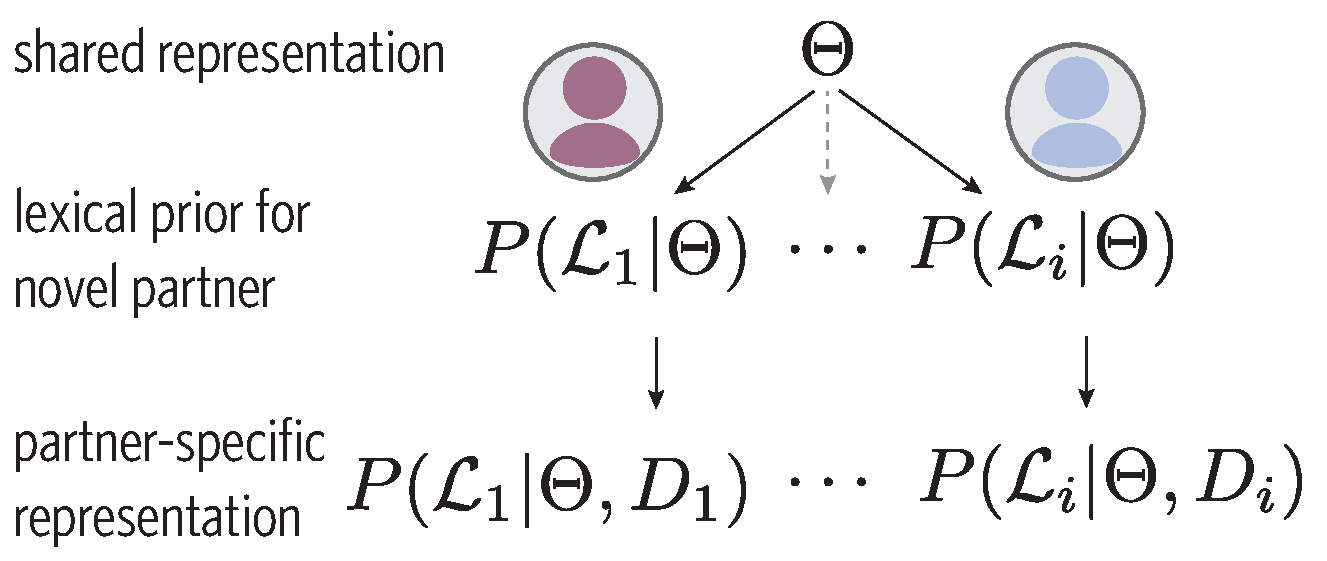
\includegraphics[scale=.45]{task1_model.pdf}
  \caption{Schematic of model}
  \label{fig:task1model}
\end{figure}
At the core of any model of referential communication is the notion of a \emph{lexicon} giving the meanings of the tokens in the language. 
We define the lexicon as a function $\mathcal{L}: (w_n, o_m) \rightarrow \mathbb{R}$, assigning any word-object pair a real-valued meaning according to how well the word $w_n$ applies to the object $o_m$. 
This is a continuous generalization of classic truth-conditional semantics \shortcite{graf_animal_2016}. 
We view the lexicon not as a lookup table or a static logical form untouched after childhood, but as a dynamic, parameterized representation that is constantly being updated.
 %\footnote{
%We mostly have nouns (\emph{poodle, animal, John}) and property adjectives (\emph{blue, squiggly, delicious}) in mind here, which can be assigned direct semantic meanings. How tricker cases like relational modifiers (\emph{some, barely, former}) are represented in the mental lexicon and how to build a fully compositional semantics from them is a topic of ongoing work in formal semantics, though see \citeA{Yildirim16_TalkerSpecificityQuantifiers} for a study exploring how these too can adapt in partner-specific ways over repeated interaction.
%}. 
%There are \emph{many} potential ways this function could be represented in the mind at the algorithmic level. It could be derived from a store of exemplars, a set of independent prototypes for each word, a neural network embedding words and objects in a vector space, and so on \cite<see>[for a recent review of candidates]{JonesEtAl15_SemanticMemory}.
At the highest level of the hierarchical lexical representation is a \emph{community-level} variable $\Theta$ parameterizing the agent's prior expectations for the likely lexicon $\mathcal{L}_i$ used by a novel community member $i$: $P(\mathcal{L}_i | \Theta)$. 
%For simple domains where the vocabulary and number of objects is small, $\Theta_0$ could simply be a $$n\times m$$ a $\times$ real-valued matrix where $n$ is the vocabulary size and $m$ is the number of objects, but for more natural tasks, it is 
%For the conceptual purposes of this paper, it is not important exactly what form this distribution takes, or what initial prior over the overhypothesis $P(\Theta_0)$ could in principle guide early language learning
%\footnote{
%For simplicity, we could assume $\Theta_0$ is an $\mathcal{W} \times \mathcal{O} \times 2$ tensor containing values $(\alpha_{(w,o)}, \beta_{(w,o)})$ for every entry $(w,o)$ in the lexicon $\mathcal{L}_i$. This would factor the lexical prior $P(\mathcal{L}_i | \Theta_0)$ into independent Beta distributions over intervals $[0,1]$. It would then be straightforward to place an uninformative prior $P(\Theta_0)$ over that tensor which does not overwhelm the likelihood \cite<see>[p. 110, for some reasonable choices]{gelman2006data}. More generally, we could allow for arbitrarily complex dependencies between entries of the lexicon by using a Bayesian neural network with weight tensor $\Theta_0$.% that takes word-object pairs $(w,o)$ as input. 
%}. It only matters that this knowledge is hierarchical: we expect all members of our language community to share some commonality in what they mean by things. 

Given observations $D_i$ from interactions with that particular individual---concretely, utterances and responses in a reference game---their \emph{partner-specific} model can be rapidly updated using Bayes rule:
$%\begin{array}{rcl}
P(\mathcal{L}_i | D_i, \Theta)  \propto P(D_i | \mathcal{L}_i) P(\mathcal{L}_i | \Theta)P(\Theta)
%                     & = & \mathbb{E}_{\Theta_0}[P(\mathcal{L}_i | \Theta_0, D_i)] 
%\end{array}
$.
%While this holds when we only have observations from a single speaker, note that our posterior beliefs about $\Theta_0$ are in fact informed by observations from \emph{all} speakers: $D = \bigcup_{i=1}^k D_i$. For  adult language users who have observed innumerable uses of language over their lifetimes, the contribution of a new data point to the overhypothesis $P(\Theta_0 | D)$ should be negligible; the contribution to a partner-specific model, however, can be quite strong. 
Additionally, because the partner-specific model depends on $\Theta$, Bayesian inference allows new data to systematically inform the shared, population-level representation as well (Fig. \ref{fig:task1model}).
Critically for predictions about generalization, new language data (i.e. particular ways of referring to the tangram shapes) may at first be more parsimoniously explained as an idiosyncratic property of a particular partner's lexicon, or ``idiolect''. 
If two or three partners all happen to use the same language, however, it starts to become more likely that a novel partner will share it as well (this transfer is sometimes referred to as ``sharing of statistical strength.'')
This formalizes the intuition from the behavioral predictions.


%In summary, our proposed hierarchical Bayesian model formalizes the intuition that global conventions are learned and generalized over many extended interactions with many different people across a lifetime, and that this shared semantic prototype is the backbone supporting rapid learning for new partners and situations. 

\subsection{Model implementation}
To implement this model, we must specify (1) the parameterization of the lexicon, (2) the linking function (i.e. likelihood function) between parameter values and observed language behavior, and (3) an algorithm to perform inference.
First, for small finite domains with $N$ words and $M$ objects, a natural parameterization of the lexicon is an $N\times M$ matrix where each cell is the value of a lexical entry, as I previously used in my dissertation work \cite{hawkins_emerging_abstractions_2018}. 
In Objective 3, we will use a neural network to extend this efficiently to arbitrarily large spaces.
Second, a natural linking hypothesis to behavior is provided by the Rational Speech Act framework, which I have helped developed throughout my dissertation work \shortcite{hawkins_why_2015,goodman_pragmatic_2016,bergen_pragmatic_2016}. 
In this framework, speakers produce utterances that are parsimonious yet informative in context with respect to their lexicon, and listeners interpret utterances by inverting a speaker model. 
Because agents expect their partner to use language rationally given some lexicon $\mathcal{L}_i$, their language use is therefore a probabilistic cue to their lexicon.
Third, we will perform inference in this model using Hamiltonian Monte Carlo (HMC) which uses gradient information to quickly converge on samples from the posterior; if HMC fails, we will use mean-field variational inference (VI), which uses stochastic gradient descent to minimize the divergence between the true posterior and a parameterized approximating family of Gaussians.

\subsection{Implementation in neural network}
Because the $N \times M$ word-object matrix used in previous Objectives cannot straightforwardly generalize to unseen words and objects and quickly becomes intractable as the vocabulary and object set grows, here we will instead take $\Theta$ to be an initialization for the weights of an image-captioning neural network (see Fig. \ref{fig:arch}A).
We will use an architecture that was introduced several years ago \shortcite{karpathy2015deep, vinyals2015show} and has become widespread in the machine learning literature.
It combines a pre-trained deep convolutional neural network (CNN) vision backbone like VGG-19 with a recurrent neural network (RNN) language module by feeding high-level CNN features into the initial hidden state of the RNN. 
While these systems are often trained end-to-end, we will freeze the weights of the vision module and isolate the language module as the site of learning in convention formation (i.e. assume that new conventions are not modifying the agent's perceptual system).
Because the Rational Speech Act framework used throughout this proposal as a linking function %for discriminative production and interpretaion in context 
has successfully been implemented on top of such CNN-RNN networks in previous work \shortcite{vedantam_context-aware_2017}, the key implementation bottleneck is not the parameterization or the linking function, but the inference algorithm.
 %We omit mathematical details here due to the conceptual nature of the article, but a full account of the non-hierarchical version of this model can be found in \citeA{hawkins_convention-formation_2017}.

While it is theoretically possible to place priors on all neural network parameters and use the same inferences techniques as above  \shortcite{joshi_personalizing_2017}, current techniques for inference in Bayesian neural networks rely on optimization of noisy gradients of variational objectives and tend not to work well. 
We will solve this problem through a novel application of recent formal insights from the Dr. Griffith's lab, which recast inference in hierarchical Bayesian models as stochastic gradient-based optimization of the more tractable model agnostic meta-learning (MAML) loss objective \cite{grant_recasting_2018}.
Finally, because maintaining full hyper-priors is costly and challenging for inference, we will assume agents only represent an \emph{empirical Bayes} point estimate of $\Theta$ \cite{gelman_bayesian_2014}.
